%%
%% Arquivo principal para:
%% - trabalhos de conclusão de curso
%%
%%NOTA: ESSE MODELO DE TCC FOI BASEADO NO MODELO DE TESE E DISSERTAÇÃO DO PPGEEC,
%%      DA UFRN,  COM  AUTORIZAÇÃO  DO  SEU  AUTOR, O PROFESSOR ADELARDO MEDEIROS
%%
%% Criado por Adelardo Medeiros, professor do Curso de Engenharia de Computação da UFRN, dezembro de 2005. 
%% Revisado pelos alunos de Metodologia da Pesquisa Científica de 2016.1, do curso de Engenharia de Computação da UFRN.
%% Adaptado por Diogo Henrique Duarte Bezerra, professor do Curso de Engenharia de Computação da UFMT, dezembro de 2020.

\documentclass[a4paper,12pt,openright,twoside]{book}

\usepackage[utf8]{inputenc}
\usepackage{ae}
\renewcommand{\familydefault}{\sfdefault}
\usepackage{pslatex}
\usepackage[portuges, brazil]{babel}
\usepackage{indentfirst}
\usepackage{graphicx}
\usepackage[portuguese,noprefix]{nomencl}
\usepackage{setspace}
\usepackage{amsmath}
\usepackage{verbatim}
\usepackage{tabularx}
\usepackage{afterpage}
\usepackage{url}
\usepackage{lib/noitemsep}
\usepackage[abbr]{lib/harvard}	
\usepackage{longtable}
\usepackage{color}
\usepackage{multirow}
\usepackage[portuguese, ruled, linesnumbered]{algorithm2e}
\usepackage{lib/capitulos}
\usepackage[breaklinks]{hyperref}
\usepackage[all]{hypcap}
\usepackage[titletoc]{appendix}
\usepackage{pdfpages}

% newcommand define novos comandos, que podem passar a ser usados da
% mesma forma que os comandos LaTeX de base.

% Implicação em fórmulas
\newcommand{\implica}{\quad\Rightarrow\quad} %Meio de linha
\newcommand{\implicafim}{\quad\Rightarrow}   %Fim de linha
\newcommand{\tende}{\rightarrow}
\newcommand{\BibTeX}{\textsc{B\hspace{-0.1em}i\hspace{-0.1em}b\hspace{-0.3em}}\TeX}

% Fração com parentesis
\newcommand{\pfrac}[2]{\left(\frac{#1}{#2}\right)}

% Transformada de Laplace e transformada Z
%\newcommand{\lapl}{\makebox[0cm][l]{\hspace{0.1em}\raisebox{0.25ex}{-}}\mathcal{L}}
\newcommand{\lapl}{\pounds}
\newcommand{\transfz}{\mathcal{Z}}

% Não aparecer o número na primeira página dos capítulos
\newcommand{\mychapter}[1]{\chapter{#1}\thispagestyle{empty}}

% Os capítulos sem número
\newcommand{\mychapterast}[1]{\chapter*{#1}\thispagestyle{empty}
\chaptermark{#1}
\afterpage{\markboth{\uppercase{#1}}{\rightmark}}
\markboth{\uppercase{#1}}{}
}

% Seções sem número
\newcommand{\mysectionast}[1]{\section*{#1}
\addcontentsline{toc}{section}{#1}
\markright{\uppercase{#1}}
}

% No tabularx, as celulas devem ser centradas verticalmente
\renewcommand{\tabularxcolumn}[1]{m{#1}}

% Células centralizadas horizontalmente no tabularx
\newcolumntype{C}{>{\centering\arraybackslash}X}

%% Abrevia figuras e tabelas
%\def\figurename{Fig.}
%\def\tablename{Tab.}


\setlength{\oddsidemargin}{3.5cm}
\setlength{\evensidemargin}{2.5cm}
\setlength{\textwidth}{15cm}
\addtolength{\oddsidemargin}{-1in}
\addtolength{\evensidemargin}{-1in}

\setlength{\topmargin}{2.0cm}
\setlength{\headheight}{1.0cm}
\setlength{\headsep}{1.0cm}
\setlength{\textheight}{22.7cm}
\setlength{\footskip}{1.0cm}
\addtolength{\topmargin}{-1in}

\bibliographystyle{bibliografia/ppgee}

\singlespacing

\makenomenclature

\begin{document}

\pagestyle{empty}

\begin{titlepage}

\begin{center}

\small

\begin{center}

\includegraphics[width=5.75cm]{pre-textuais/figuras/brasao-republica.jpeg}    
\end{center}

\LARGE{\textbf{MINISTÉRIO DA EDUCAÇÃO\\
UNIVERSIDADE FEDERAL DE MATO GROSSO\\}}

\vfill

\LARGE

\textbf{Relatório Final do Projeto de Pesquisa}

\vfill

\Large

Projeto DDR - Dashboard of Data Reconciliation

\vfill

\large

Coordenador de Pesquisa: João Gustavo Coelho Pena

\vfill

\large

Cuiabá, MT, 27 de Setembro de 2024

\end{center}

\end{titlepage}


\doublespacing

\begin{center}
    \LARGE PROPOSTA DE PROJETO DE PESQUISA 
    \normalsize 
\end{center}

\vspace{1cm}

\textbf{Titulo do Projeto:} "DDR - DASHBOARD OF DATA RECONCILIATION"

\vspace{1cm}

\textbf{Linha de Pesquisa:} Computalção

\vspace{1cm}

\textbf{Equipe Técnica:}

\vspace{0.5cm}

\textbf{Coordenador de Pesquisa:} João Gustavo Coelho Pena

\vspace{0.5cm}

\textbf{Orientadores:} 

- João Gustavo Coelho Pena

- Gustavo Post Sabin

\vspace{0.5cm}

\textbf{Orientandos (estudantes de graduaçõ):} 

- Nilton Aguiar dos Santos (RGA: 201811901022) - curso Eng. de Computação 


\mychapterast{Resumo}

Este Trabalho trata-se do Relatório Final do Projeto de Pesquisa intitulado "Projeto DDR – DASHBOARD OF DATA RECONCILIATION", nele é descrito os principais fundamentos, informações, metodologias e resultados alcançados.  

O Projeto DDR é um \textit{software online} voltado para reconciliação e qualidade de dados, utilizando técnicas de minimização de funções multivariáveis pelo método dos multiplicadores de Lagrange. A solução prioriza uma abordagem baseada na \textit{web}, oferecendo ao usuário a capacidade de realizar a análise e reconciliação de dados de forma remota e eficiente, com foco nos conceitos computacionais modernos, para proporcionar uma experiência facilitada. O \textit{software} aplica cálculos matemáticos e estatísticos ao longo de todo o processo, especificamente voltados para problemas de reconciliação de dados.

Por meio do DDR, é possível modelar todo um processo industrial, alimentá-lo com dados oriundos da planta em questão e, a partir disso, reconciliar e verificar a qualidade dos dados em tempo real. O \textit{software} se destaca como uma solução inovadora, pois não há concorrente direto que ofereça as mesmas funcionalidades em um ambiente mais acessível e ágil no estado de Mato Grosso. Ao longo deste trabalho, são detalhados o processo filosófico de desenvolvimento, os cálculos matemáticos, os conceitos estatísticos e computacionais, e a lógica do \textit{software} aplicada como solução. Exemplos do código funcional e considerações finais sobre o trabalho realizado são apresentados nos capítulos finais.

\vspace{1.5ex}

{\bf Palavras-chave}: CSS; \textit{Dashboard}; Desenvolvimento \textit{Web}; Desenvolvimento de \textit{Software}; HTML; Indústria 4.0; Javascript; Multiplicadores de Lagrange; Qualidade de Dados; Python; Reconciliação de Dados.




\frontmatter

\phantomsection
\addcontentsline{toc}{chapter}{Sumário}
\tableofcontents

\cleardoublepage
\phantomsection
\addcontentsline{toc}{chapter}{Lista de Figuras}
\listoffigures

\mainmatter
\pagestyle{headings}

\mychapter{Apresentação da Inovação Científica}
\label{Apresentacao}

No Capítulo \Ref{Apresentacao} será feita a apresentação do trabalho produzido, introduzindo os fundamentos da solução proposta, aqui denominada \textbf{DDR} (\textit{Dashboard of Data Reconciliation}), que visa proporcionar uma plataforma inovadora para a reconciliação e análise de dados industriais, com ênfase na facilidade de manuseabilidade e adaptação à ferramenta DDR.

\section{Problematização}

A reconciliação de dados em processos industriais no Brasil sempre representou um desafio para a garantia de qualidade e confiabilidade das informações coletadas \cite{datarecshakar}. O setor industrial brasileiro frequentemente enfrenta imprecisões em dados provenientes de sensores e equipamentos utilizados em plantas industriais \cite{produtividadeindustria}. Tais imprecisões, derivadas de erros aleatórios ou sistemáticos nas medições, comprometem a eficiência operacional e dificultam a tomada de decisões estratégicas \cite{datarecsurvey}. A ausência de ferramentas ágeis e acessíveis, capazes de realizar a reconciliação de dados em tempo real ou em bateladas, impacta negativamente a competitividade das indústrias nacionais \cite{industry4status}.

Além disso, há uma notável carência no mercado nacional de soluções tecnológicas que integrem processos industriais complexos de forma eficaz, combinando uma interface de fácil uso com a capacidade de processamento de dados em larga escala \cite{danielhoduin}. As soluções disponíveis no mercado brasileiro frequentemente apresentam custos elevados e dependem de infraestrutura local robusta, tornando-se inviáveis para pequenas e médias empresas \cite{industryinternet}. 

Portanto, a inovação tecnológica apresentada visa superar essas limitações por meio de uma plataforma \textit{online} acessível, eficiente e escalável, projetada para atender às necessidades específicas das indústrias brasileiras e contribuir para seu desenvolvimento e crescimento sustentável \cite{reconset}.

\section{Metas}

A inovação teve como principais metas, cada uma delas detalhada a seguir para esclarecer as direções e objetivos específicos do projeto:

\subsection{Desenvolver uma ferramenta online}

O desenvolvimento de uma ferramenta inteiramente \textit{online} foi um dos pilares centrais do DDR \cite{bilco}. O objetivo dessa meta foi garantir que o sistema pudesse ser acessado remotamente, sem a necessidade de instalação de \textit{software} ou infraestrutura física complexa. Ao optar por uma solução baseada na \textit{web}, o DDR oferece alta acessibilidade para diversas indústrias, independentemente da localização geográfica ou dos recursos tecnológicos disponíveis localmente \cite{industrynew}. A utilização de tecnologias \textit{web} modernas permite que o sistema funcione de maneira eficaz em uma variedade de dispositivos e plataformas, garantindo facilidade de acesso e manutenção simplificada \cite{javascriptframework}. Essa abordagem também reduz custos operacionais, já que elimina a necessidade de \textit{hardware} dedicado ou suporte técnico especializado para implementação.

\subsection{Desenvolver uma interface responsiva}

Uma das principais metas do DDR foi garantir que a interface de usuário fosse responsiva, intuitiva e amigável \cite{frontendperfomance}. Isso significa que a plataforma foi projetada para proporcionar uma experiência de uso fluida, tanto para operadores industriais quanto para engenheiros de processos, ao modelar fluxos e simulações de processos industriais \cite{reactjs}. A interface desenvolvida em \textit{React.js} permite a manipulação visual de processos, utilizando gráficos e fluxogramas que facilitam a compreensão dos dados e das variáveis envolvidas \cite{eloquentjavascript}. A criação de uma experiência de usuário simples e intuitiva foi fundamental para garantir que a plataforma fosse amplamente adotada, mesmo por usuários com pouca experiência prévia em sistemas de reconciliação de dados.

\subsection{Desenvolver a reconciliação de dados em bateladas}

O DDR foi desenvolvido com a capacidade de realizar reconciliação de dados em bateladas \cite{reconset}. Essa funcionalidade é essencial para ambientes industriais que operam em ciclos discretos, onde os dados podem ser coletados e reconciliados ao final de cada ciclo de produção \cite{danielhoduin}. A reconciliação em bateladas permite a correção e o ajuste dos dados medidos após o término de uma operação, garantindo que os resultados respeitem as leis de conservação de massa e energia \cite{balancecontrol}. Este tipo de reconciliação é particularmente útil para plantas industriais que operam com grandes volumes de dados acumulados durante um intervalo de tempo, permitindo uma análise detalhada e precisa dos dados ao final de cada batelada \cite{datarecshakar}.

\subsection{Desenvolver a reconciliação de dados em tempo real}

Além da reconciliação em bateladas, o DDR também foi projetado para realizar reconciliação de dados em tempo real \cite{datarecshakar}. Essa funcionalidade é especialmente relevante para plantas industriais que operam continuamente, exigindo correções imediatas nos dados coletados, permitindo uma resposta rápida às variações do processo \cite{danielhoduin}. A reconciliação em tempo real ajusta os dados à medida que são coletados, corrigindo erros de medição conforme ocorrem, aumentando assim a precisão dos dados usados para controle e monitoramento dos processos em tempo real \cite{reformulationdatarecon}. Essa capacidade é crucial para garantir a eficiência operacional e evitar decisões baseadas em dados imprecisos, aprimorando o controle dos processos industriais e otimizando o desempenho geral da planta \cite{computecontrol}.

\mychapter{Processos ou Produtos Tecnológicos Inovadores Gerados} \label{Cap
}

O Capítulo \ref{Cap
} descreve os produtos tecnológicos inovadores gerados a partir da pesquisa, com ênfase no desenvolvimento e aplicação do DDR.

\section{Descrição do Projeto DDR}

\subsection{Finalidade e Implementação}

O DDR é uma plataforma \textit{online} projetada para a reconciliação de dados em processos industriais, com o objetivo de melhorar a precisão e confiabilidade das informações obtidas a partir de sensores \cite{datarecshakar}. O sistema visa corrigir erros de medição, garantindo que os dados estejam em conformidade com as leis de conservação, como a de massa e energia, utilizando o \textbf{método dos multiplicadores de Lagrange}, amplamente utilizado em problemas de otimização multivariável \cite{optimizationlagrange}. A reconciliação de dados robusta garante que informações inconsistentes sejam ajustadas, elevando a qualidade dos dados utilizados para controle e otimização dos processos produtivos \cite{datarecragnoli}.

\subsection{Arquitetura e Tecnologias Utilizadas}

A arquitetura do DDR foi desenvolvida para garantir escalabilidade e eficiência. O \textit{front-end} foi implementado com \textbf{React.js}, uma biblioteca popular para o desenvolvimento de interfaces dinâmicas e responsivas, oferecendo uma experiência de usuário fluida, adequada para o monitoramento em tempo real \cite{reactjs}.

O \textit{back-end}, implementado em \textbf{Python}, utiliza o \textbf{Flask} para gerenciamento de servidor, oferecendo uma arquitetura leve e eficiente. Para cálculos matemáticos e otimizações, o sistema integra bibliotecas como \textbf{NumPy} e \textbf{SciPy}, que fornecem suporte avançado para operações numéricas e permitem a implementação do método dos multiplicadores de Lagrange \cite{lagrangehistory}. O banco de dados escolhido foi o \textbf{PostgreSQL}, garantindo a integridade e escalabilidade necessárias para o armazenamento de grandes volumes de dados industriais \cite{databasesqlmaster}.

A plataforma também se destaca pelo uso de \textbf{ReactFlow}, uma ferramenta visual que facilita a criação de diagramas interativos, permitindo que os operadores monitorem fluxos de materiais e energia, identifiquem padrões e detectem possíveis falhas de maneira rápida e eficiente \cite{graph}. Esses diagramas fornecem uma representação visual clara dos processos industriais, o que é essencial para a tomada de decisões operacionais \cite{frontendperfomance}.

\section{Área Estratégica Atingida e Benefícios ao Setor Industrial}

O DDR está em sintonia com os princípios da \textbf{Indústria 4.0}, que busca aumentar a eficiência e competitividade das empresas por meio da digitalização e automação dos processos produtivos \cite{industry4}. A plataforma contribui diretamente para a automação de processos e o aprimoramento do controle de qualidade, facilitando a integração de dados de sensores e dispositivos IoT, o que gera um ambiente de produção mais eficiente e preciso \cite{industryiot}.

Entre os principais benefícios trazidos pela implementação do DDR no setor industrial estão a redução de custos operacionais, a diminuição de tempos de inatividade e a melhora significativa na eficiência do controle de processos \cite{industryinternet}. A plataforma também é altamente escalável, podendo ser aplicada em diferentes tipos de indústrias, independentemente de seu porte, o que a torna uma ferramenta adaptável a um mercado industrial em constante evolução \cite{industrybuild}.

Além disso, ao garantir a consistência e a precisão dos dados, o DDR contribui para um ambiente produtivo mais sustentável, minimizando desperdícios e otimizando o uso de recursos \cite{industrydigital}. Isso reflete diretamente na competitividade das indústrias brasileiras, que poderão adotar as melhores práticas de automação e digitalização para se adequar às exigências da Indústria 4.0 \cite{industrychina}.
\mychapter{Marco Teórico}
\label{Cap:MarcoTeorico}

O Capítulo \ref{Cap:MarcoTeorico} apresenta os principais conceitos teóricos que embasam o desenvolvimento da plataforma DDR, focando na reconciliação de dados por meio do método dos multiplicadores de Lagrange e na utilização de tecnologias \textit{web} no contexto da automação industrial.

\section{Reconciliação de Dados e o Método dos Multiplicadores de Lagrange}

A \textit{reconciliação de dados} é uma técnica essencial para garantir a consistência e a precisão das informações coletadas por sensores em processos industriais \cite{datarecshakar}. Esse método visa minimizar os erros sistemáticos e aleatórios que comumente afetam as medições industriais, corrigindo as inconsistências nos dados coletados \cite{datarecragnoli}. A reconciliação de dados assegura que os resultados obtidos respeitem as leis de conservação, como a conservação de massa e energia, o que é crucial para a operação otimizada de plantas industriais \cite{balancecontrol}.

O DDR utiliza o \textit{método dos multiplicadores de Lagrange} como base para seu sistema de reconciliação de dados \cite{optimizationlagrange1982}. Esse método matemático é amplamente empregado para resolver problemas de otimização multivariável com restrições, ajustando os valores medidos de modo a atender a equações de balanço \cite{computecontrol}. Em um contexto industrial, a aplicação dos multiplicadores de Lagrange permite que os dados reconciliados estejam em conformidade com as leis físicas, minimizando desvios nas medições e proporcionando resultados mais confiáveis para processos críticos \cite{danielhoduin}. Essa técnica oferece uma solução robusta, garantindo que as indústrias operem com dados precisos e consistentes, o que é vital para processos de otimização e controle \cite{reformulationdatarecon}.

\section{Tecnologias \textit{Web} no Contexto da Automação Industrial}

A automação industrial moderna depende de tecnologias que permitem a integração de dados e o monitoramento em tempo real. O DDR foi projetado utilizando tecnologias \textit{web} avançadas que tornam a plataforma escalável e acessível de forma remota, atendendo às exigências da \textit{Indústria 4.0} \cite{webusage}. 

No \textit{front-end}, a escolha de \textbf{React.js} proporciona uma interface de usuário altamente responsiva, capaz de atualizar automaticamente as informações recebidas em tempo real. Essa tecnologia oferece uma experiência de uso eficiente e intuitiva, necessária para lidar com os fluxos de dados contínuos que são comuns em ambientes industriais \cite{reactjs}. A interatividade e reatividade proporcionadas por essa tecnologia tornam a plataforma ideal para o monitoramento e controle visual de processos industriais \cite{eloquentjavascript}.

No \textit{back-end}, a escolha do \textbf{Python} como linguagem de desenvolvimento se deve à sua robustez e capacidade de lidar com grandes volumes de dados de forma eficiente \cite{databasesql}. O uso de bibliotecas como \textbf{AsyncIO} e \textbf{FastAPI} permite que o \textit{back-end} do DDR processe dados de forma assíncrona, oferecendo suporte para múltiplas fontes de dados e garantindo a escalabilidade do sistema \cite{backenddevroles}. Essa arquitetura assíncrona é fundamental para manter a integridade dos dados em tempo real sem comprometer o desempenho do sistema \cite{industrydigital}.

Para a visualização dos fluxos de dados e a modelagem dos processos industriais, o DDR incorpora a biblioteca \textbf{ReactFlow}. Essa ferramenta permite a criação de diagramas interativos que facilitam a compreensão dos fluxos de materiais e a identificação de anomalias, padrões ou falhas nos processos industriais \cite{graph}. A visualização clara e interativa dos dados é essencial para que operadores e engenheiros tomem decisões rápidas e informadas, otimizando os processos produtivos.

Assim, o DDR se posiciona como uma solução alinhada às demandas da \textit{Indústria 4.0}, integrando tecnologias \textit{web} modernas com técnicas avançadas de reconciliação de dados, oferecendo às indústrias brasileiras uma ferramenta poderosa para automação e otimização de processos \cite{industry4status}.

\mychapter{Procedimentos Metódicos}
\label{Cap:ProcedimentosMetodicos}

O Capítulo \ref{Cap:ProcedimentosMetodicos} descreve os procedimentos metodológicos adotados no desenvolvimento da plataforma DDR, detalhando as etapas do processo de implementação, as ferramentas e tecnologias utilizadas, e os métodos aplicados para garantir a qualidade e eficiência do sistema.

\section{Desenvolvimento do Sistema DDR}

O desenvolvimento da plataforma DDR foi realizado seguindo uma abordagem iterativa e incremental, baseada no método ágil \textit{Scrum}. Essa abordagem permitiu uma adaptação constante às necessidades do projeto, com entregas frequentes e revisões contínuas, assegurando que o sistema atendesse aos requisitos funcionais e não funcionais previamente estabelecidos.

\subsection{Arquitetura do Sistema}

A arquitetura do DDR foi projetada para garantir escalabilidade, modularidade e alto desempenho. O sistema foi desenvolvido utilizando uma arquitetura cliente-servidor, com o \textit{front-end} e o \textit{back-end} sendo implementados separadamente, garantindo uma maior flexibilidade e manutenibilidade.

O \textit{front-end} foi implementado utilizando a biblioteca \textbf{React.js}, que oferece uma interface de usuário dinâmica e responsiva, capaz de lidar com a visualização de grandes volumes de dados em tempo real. A arquitetura \textbf{React} baseada em componentes permitiu a reutilização de código, tornando o sistema mais modular e facilitando a manutenção e escalabilidade. O desenvolvimento da solução foi aprimorada com a utilização de \textbf{TypeScript}, um \textit{superset} ao JavaScript que oferece tipagem estática, garantindo maior segurança e previsibilidade no desenvolvimento.

O \textit{back-end} foi desenvolvido utilizando \textbf{Python}, o que permitiu uma implementação eficiente, especialmente em relação ao processamento assíncrono de grandes volumes de dados industriais. O uso de \textbf{FastAPI}, uma \textit{framework} moderna para a criação de APIs RESTful, garantiu a comunicação rápida e segura entre o \textit{front-end} e o \textit{back-end}. O Python também foi utilizado para a execução dos cálculos de reconciliação de dados, aproveitando bibliotecas como \textbf{NumPy} e \textbf{SciPy} para a resolução de problemas de otimização multivariáveis.

\subsection{Modelagem e Reconciliação de Dados}

A reconciliação de dados foi implementada com base no \textbf{método dos multiplicadores de Lagrange}, que é amplamente utilizado para resolver problemas de otimização multivariáveis com restrições. Este método foi aplicado para ajustar os dados de medição provenientes dos sensores industriais, assegurando que os resultados estivessem em conformidade com as leis de conservação de massa e energia.

Durante o processo de reconciliação, os dados de entrada eram validados e ajustados de forma a minimizar os erros sistemáticos e aleatórios presentes nas medições. A aplicação deste método foi crucial para garantir a consistência dos dados e a confiabilidade dos resultados, especialmente em ambientes industriais onde medições imprecisas podem comprometer a eficiência dos processos produtivos.

\section{Ferramentas Utilizadas no Desenvolvimento}

\subsection{React.js e TypeScript no Front-End}

O \textbf{React.js} foi escolhido para o desenvolvimento da interface do DDR devido à sua eficiência no gerenciamento de interfaces dinâmicas e na manipulação de grandes volumes de dados em tempo real. Sua arquitetura baseada em componentes reutilizáveis facilitou a manutenção do sistema e garantiu escalabilidade, essenciais para o ambiente industrial. A adoção de \textbf{TypeScript} acrescentou uma camada adicional de segurança, permitindo a detecção de erros durante o desenvolvimento e aumentando a confiabilidade e robustez do código.

\begin{figure}[htbp!]
    \begin{center}
        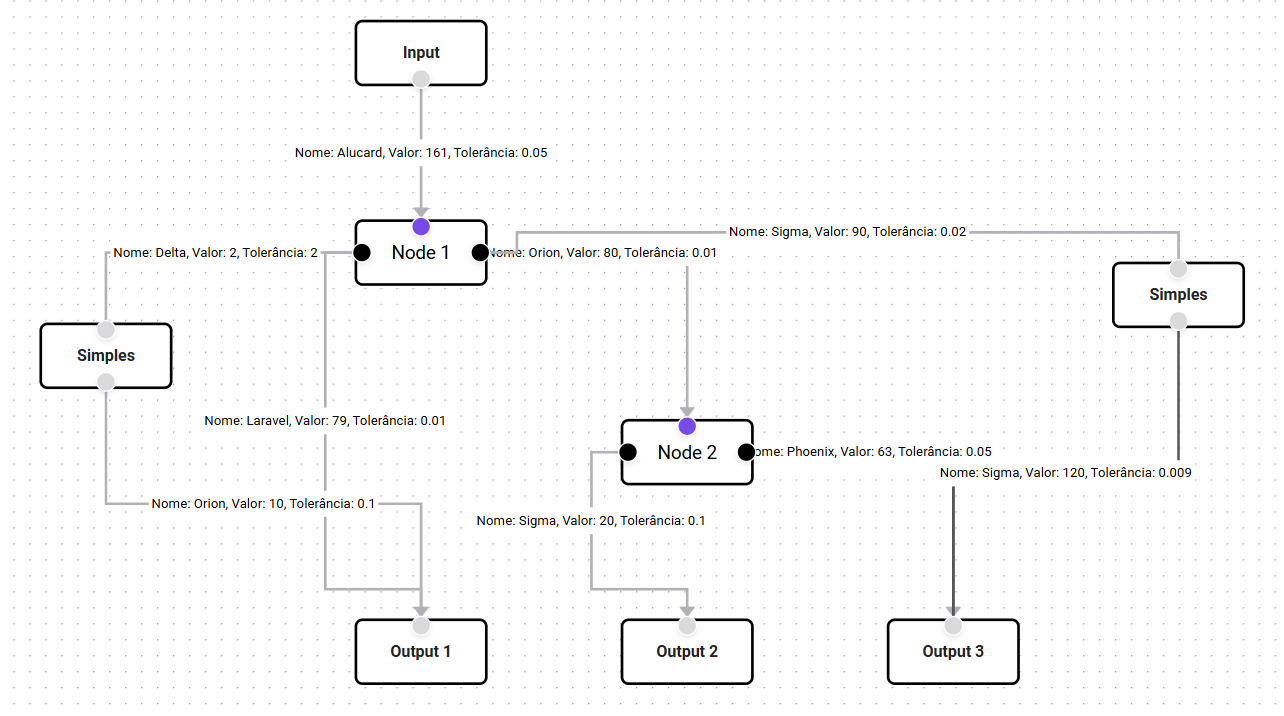
\includegraphics[width=0.75\textwidth]{figuras/reactflow.png}
        \caption{Exemplo de uma modelagem com o ReactFlow.}
        \label{fig:ReactFlowPicture}
    \end{center}
\end{figure}

Um elemento crucial no \textit{front-end} foi a utilização da biblioteca \textbf{ReactFlow}, especializada na criação de diagramas interativos. Ela proporcionou uma visualização clara dos fluxos de dados industriais, permitindo que operadores e engenheiros modelassem e monitorassem processos complexos diretamente na interface do DDR. A biblioteca foi adaptada com diversas funcionalidades personalizadas, como a extração de matrizes de incidência das conexões entre nódulos, facilitando a análise das relações entre variáveis industriais.

Essas adaptações permitiram que o ReactFlow atendesse às demandas específicas da modelagem industrial, tornando-o uma ferramenta eficiente para o controle visual de processos.

\subsection{Python no Back-End}

O \textbf{Python} foi escolhido para o \textit{back-end} do DDR devido à sua flexibilidade e eficiência no processamento de grandes volumes de dados e operações assíncronas. A combinação de \textbf{FastAPI} com \textbf{NumPy} permitiu a execução eficiente de cálculos complexos, essenciais para os processos de reconciliação de dados, enquanto o \textbf{SQLAlchemy} foi utilizado para gerenciar a comunicação com o banco de dados \textbf{PostgreSQL}, garantindo integridade e performance nas operações de leitura e escrita.

A arquitetura do \textit{back-end} foi projetada com base no \textit{framework} \textbf{Flask}, criando um servidor leve e escalável, com três rotas principais em padrão RESTful:

\begin{itemize}
    \item \textbf{/reconcile}: Responsável por processar os dados de reconciliação. O cliente pode enviar tanto dados em tempo real quanto em bateladas para que o servidor aplique os algoritmos de reconciliação e retorne os dados corrigidos, o qual se comunica com as funções de minimização de multivariáveis aplicando o método de Lagrange.
    \item \textbf{/reconciled\_data}: Realiza consultas ao banco de dados \textbf{PostgreSQL} para recuperar e fornecer ao cliente os dados já reconciliados, garantindo o acesso contínuo às informações processadas.
    \item \textbf{/health}: Verifica o \textit{status} do sistema, monitorando a saúde do servidor e sua conexão com o banco de dados, assegurando a estabilidade e disponibilidade da plataforma.
\end{itemize}

Essa arquitetura permite uma integração eficiente entre o \textit{front-end} e o \textit{back-end}, garantindo a escalabilidade e o desempenho da plataforma em ambientes industriais complexos.


\subsection{Banco de Dados PostgreSQL}

O \textbf{PostgreSQL} foi adotado no DDR devido à sua robustez, escalabilidade e adequação ao gerenciamento de grandes volumes de dados industriais. Sua capacidade de lidar com consultas complexas e realizar operações matemáticas avançadas torna-o ideal para armazenar e processar dados contínuos provenientes de sensores industriais, garantindo integridade e segurança nas operações de reconciliação.

A eficiência do \textbf{PostgreSQL} é reforçada por seus recursos avançados de indexação, como \textit{B-tree} e \textit{hash indexes}, que permitem uma rápida recuperação de dados, otimizando consultas complexas e cálculos em grandes matrizes sem comprometer o desempenho do sistema.

A estrutura de dados no banco foi projetada para garantir integridade e rastreabilidade, com a tabela principal de reconciliação contendo as seguintes colunas:

\begin{itemize}
    \item \textbf{id}: Chave primária única para identificar cada registro.
    \item \textbf{user}: Identificação do usuário que realizou a reconciliação, garantindo rastreamento e auditoria.
    \item \textbf{time}: Armazena a data e hora da reconciliação, crucial para a análise histórica e monitoramento contínuo.
    \item \textbf{tagname}: Nome da tag do sensor ou medidor que originou os dados.
    \item \textbf{tagreconciled}: Valor da variável após a reconciliação, ajustado para conformidade com as leis de conservação.
    \item \textbf{tagcorrection}: Valor da correção aplicada ao dado original, refletindo o ajuste necessário.
    \item \textbf{tagmatrix}: Matriz de ajuste aplicada, essencial para garantir consistência com as leis de conservação.
\end{itemize}

A adoção do \textbf{PostgreSQL} garante a segurança e eficiência no armazenamento e recuperação dos dados processados, permitindo que o sistema DDR atenda às exigências de alta quantidade de dados e confiabilidade destes em ambientes industriais.

\mychapter{Resultados}
\label{Cap:Resultados}

A plataforma \textbf{DDR} foi desenvolvida para reconciliar dados industriais de forma eficaz, corrigindo inconsistências e aumentando a precisão dos processos produtivos. Utilizando as tecnologias \textit{React.js}, \textit{Python} e \textit{ReactFlow}, a interface da plataforma se mostrou escalável e interativa, adequada para o monitoramento em tempo real de grandes volumes de dados.

A Figura \ref{fig:ReactFlowPicture} ilustra o resultado final da interface do cliente, que oferece uma visualização clara dos fluxos de dados industriais.

\begin{figure}[htbp!]
    \begin{center}
        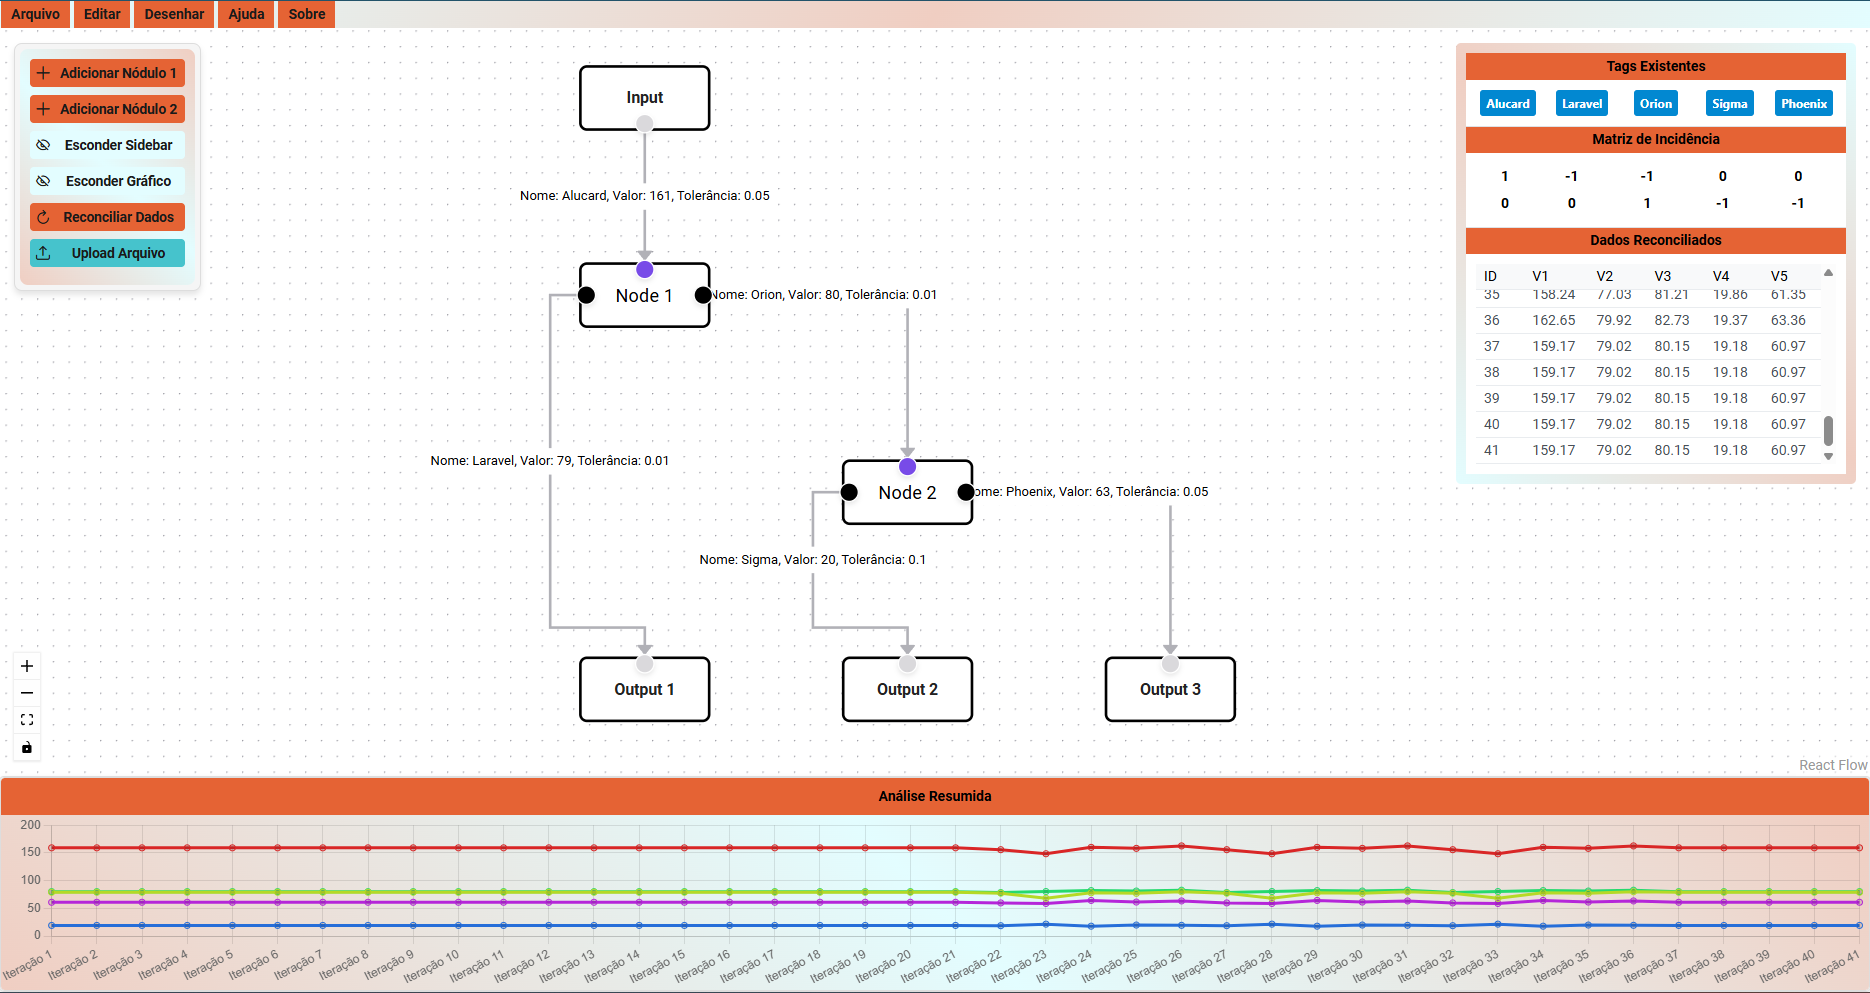
\includegraphics[width=0.75\textwidth]{figuras/principal.png}
        \caption{Interface final do cliente DDR.}
        \label{fig:ReactFlowPicture}
    \end{center}
\end{figure}

O sistema demonstrou excelente desempenho no processamento de grandes volumes de dados, utilizando as bibliotecas \textbf{NumPy} e \textbf{SciPy} para realizar cálculos complexos. O banco de dados \textbf{PostgreSQL} foi responsável por garantir a integridade dos dados e a eficiência nas consultas e operações, mesmo em cenários de alta demanda.

A reconciliação de dados em bateladas foi completamente implementada, corrigindo dados de sensores com base em leis de conservação de massa e energia. O sistema se mostrou eficaz em ajustar os dados brutos, eliminando erros e fornecendo informações consistentes para otimização de processos industriais.


\mychapter{Considerações Finais}
\label{Cap:ConsideracoesFinais}

O desenvolvimento da plataforma DDR foi bem-sucedido, atingindo a maior parte dos objetivos inicialmente propostos, especialmente no que se refere à melhoria da consistência e qualidade dos dados industriais por meio da aplicação de métodos avançados como os multiplicadores de Lagrange. O uso de tecnologias modernas, como \textit{React.js}, \textit{Python} e \textit{ReactFlow}, foi fundamental para a criação de uma interface \textit{web} escalável, eficiente e intuitiva, adequada para o monitoramento e controle de processos industriais em tempo real e a interface final do cliente foi capaz de proporcionar uma visualização clara e interativa dos fluxos de dados industriais.

Para o futuro, a plataforma DDR tem grande potencial para expansão e melhorias. A incorporação de ferramentas de \textbf{predição de comportamento}, com o uso de \textit{machine learning}, poderia proporcionar \textit{insights}, permitindo a detecção antecipada de falhas, otimização de manutenção preventiva e identificação de padrões anômalos nos dados reconciliados. Esse avanço agregaria um valor significativo à plataforma, transformando-a em uma ferramenta proativa na gestão de processos industriais.

Além disso, aprimoramentos na interface, como a adição de \textbf{ferramentas de análise avançada}, gráficos interativos e \textit{dashboards} personalizáveis com alertas automáticos, poderiam melhorar ainda mais a usabilidade e eficiência do sistema. Esses recursos facilitariam o monitoramento contínuo, permitindo respostas rápidas a condições críticas e melhorando a eficácia operacional.

Outro ponto importante seria a expansão da integração com sistemas de gestão como ERP e SCADA. A comunicação direta entre os dados reconciliados e as plataformas de gestão estratégica permitiria uma maior automação e sincronização dos processos industriais, otimizando a tomada de decisões.
Outro ponto importante seria a expansão da integração com sistemas de gestão como ERP e SCADA. A comunicação direta entre os dados reconciliados e as plataformas de gestão estratégica permitiria uma maior automação e sincronização dos processos industriais, otimizando a tomada de decisões.

Com essas melhorias, o DDR tem o potencial de se consolidar como uma ferramenta indispensável na \textit{Indústria 4.0}, não apenas facilitando a reconciliação de dados, mas também oferecendo \textbf{insights} preditivos e maior automação. Assim, a plataforma se posiciona como uma base sólida para inovações futuras no setor industrial, contribuindo para o avanço tecnológico e o aumento da competitividade das indústrias.

\phantomsection
\addcontentsline{toc}{chapter}{Referências bibliográficas}
\bibliography{bibliografia/bibliografia}

% \begin{appendices}
% \appendix
% %%
%% Apêndice
%%

\mychapter{Tabelas Completas}
\label{Cap:apendiceA}

Todas as tabelas que são grandes demais para serem incluídas no texto estão apresentadas neste apêndice.

\section{Tabela de requisitos funcionais}

\begin{longtable}{| p{.15\textwidth} | p{.40\textwidth} | p{.15\textwidth} |  p{.15\textwidth} |} \hline
\textbf{Identificador} & 
\textbf{Descrição} & 
\textbf{Prioridade} & 
\textbf{Requisitos Relacionados} \\ \hline
RF01 & 
O sistema deve permitir que os usuários modelarem a dinâmica dos sensores presentes em uma planta industrial. & 
Alta & 
RF02 \\ \hline
RF02 &
Os usuários devem ser capazes de alimentar o sistema com os dados gerados pelos sensores. &
Alta &
RF01 \\ \hline
RF03 & 
O sistema deve oferecer uma interface de usuário intuitiva e acessível. 
& Média 
& - \\ \hline
RF04 & 
O sistema deve realizar cálculos de reconciliação de dados de forma ágil e rápida. & 
Alta & 
RF01, RF02 \\ \hline
RF05 & 
O sistema deve garantir a compatibilidade de dados, mesmo com formatos heterogêneos. & 
Alta & 
RF01, RF02, RF03 \\ \hline
RF06 & 
Os usuários devem poder exportar os resultados da reconciliação de dados para diferentes formatos de arquivo. & 
Média &
RF01, RF02, RF03, RF04, RF05 \\ \hline
RF07 & 
O sistema deve permitir aos usuários configurar alertas para notificar sobre eventos importantes relacionados aos dados dos sensores. & 
Alta & 
RF01, RF02 \\ \hline
RF08 
& O sistema deve fornecer funcionalidades de visualização de dados em tempo real, incluindo gráficos e relatórios personalizáveis. &
Alta &
RF02, RF05 \\ \hline
RF09 & 
O sistema deve permitir a integração com outros sistemas de monitoramento industrial, facilitando a troca de dados e informações. & 
Alta & 
RF05, RF06 \\ \hline
\caption{Tabela completa dos requisitos funcionais do \textit{software}.}
\label{tab:apendice_req_funcionais}
\end{longtable}

\section{Tabela de requisitos não funcionais}

\begin{longtable}
{| p{.15\textwidth} | p{.55\textwidth} | p{.15\textwidth} |} 
    \hline
    \textbf{Identificador} & \textbf{Descrição} & \textbf{Prioridade} \\
    \hline
    RNF01 & O sistema deve ser altamente escalável para lidar com um grande volume de dados de sensores. & Alta \\
    \hline
    RNF02 & A segurança dos dados deve ser uma prioridade, garantindo proteção contra acesso não autorizado e manipulação indevida. & Alta \\
    \hline
    RNF03 & O desempenho do sistema deve ser otimizado para garantir tempos de resposta rápidos, mesmo em momentos de pico de uso. & Alta \\
    \hline
    RNF04 & O sistema deve ser facilmente configurável e customizável para atender às necessidades específicas de diferentes ambientes industriais. & Média \\
    \hline
    RNF05 & A manutenibilidade do sistema deve ser uma consideração fundamental, facilitando atualizações, correções de bugs e modificações futuras. & Média \\
    \hline
    RNF06 & A usabilidade do sistema deve ser intuitiva, permitindo uma curva de aprendizado mínima para os usuários. & Média \\
    \hline
    RNF07 & O sistema deve ser compatível com diferentes navegadores, garantindo sua acessibilidade em uma variedade de ambientes de implantação. & Alta \\
    \hline
    RNF8 & O sistema deve estar em conformidade com regulamentações de privacidade de dados, como GDPR, garantindo o tratamento adequado e a proteção das informações pessoais dos usuários. & Alta \\
    \hline
    RNF9 & A tolerância a falhas do sistema deve ser implementada, garantindo a continuidade das operações mesmo em caso de falhas de componentes individuais. & Alta \\
    \hline
    RNF10 & O tempo de resposta do sistema deve ser consistente e previsível, independentemente da carga de trabalho ou do número de usuários simultâneos. & Média \\
    \hline
\caption{Tabela de Requisitos Não Funcionais} % needs to go inside longtable environment
\label{tab:apendice_req__naofuncionais}
\end{longtable}
% \end{appendices}

% \renewcommand{\appendixname}{Anexo}
% \begin{appendices}
% \appendix
% % %%
% %% Anexo
% %%

% \mychapter{Termo de Autorização do Autor}
% \label{Cap:anexo}

% A principal diferença entre anexo e apêndice é que os apêndices são textos criados pelo próprio autor para complementar sua argumentação, enquanto os anexos são documentos criados por terceiros e usados pelo autor.

% Tanto o apêndice quanto o anexo devem estar presentes no sumário dos trabalhos científicos. Os apêndices devem aparecer depois das referências e os anexos depois dos apêndices.

% 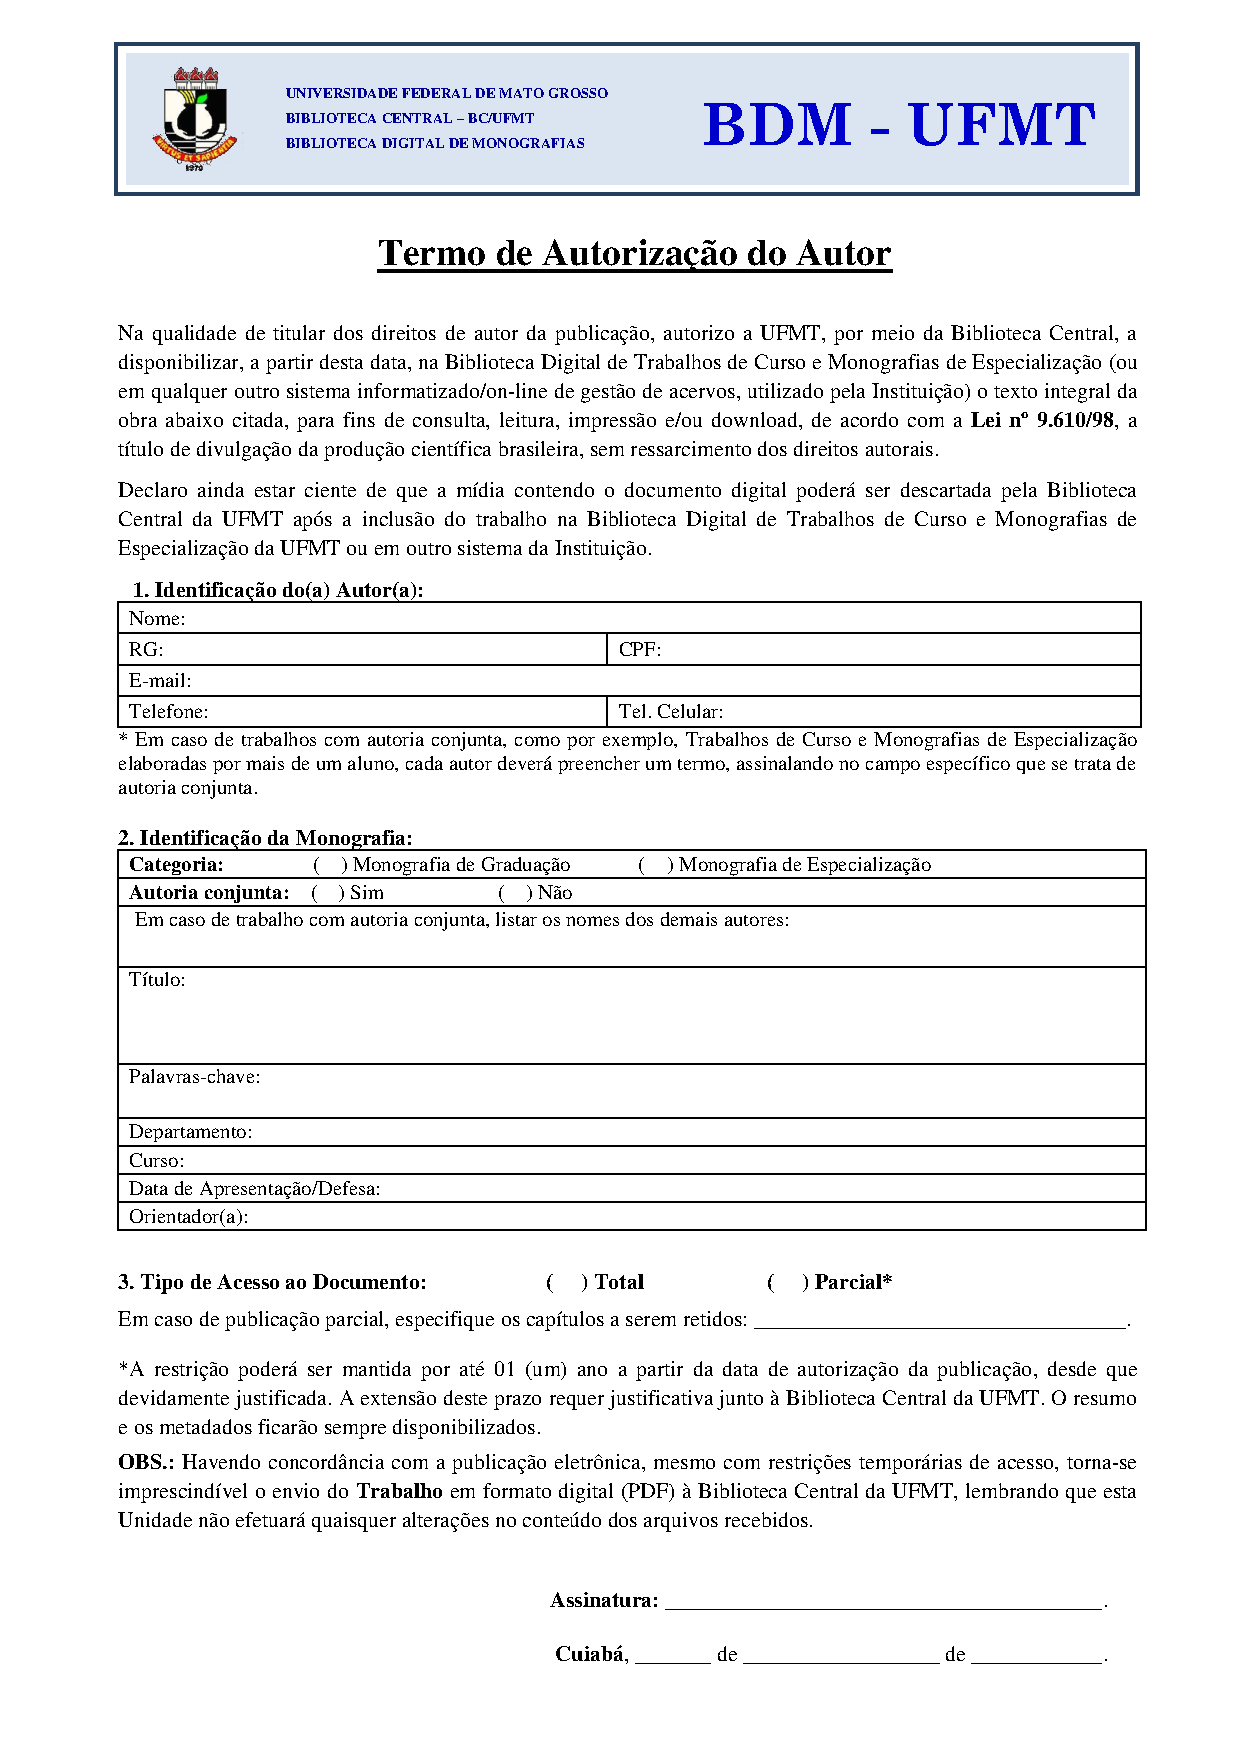
\includepdf[pages=-]{textuais/anexo/termo_de_autorizacao.pdf}

% \end{appendices}

\end{document}
